\documentclass[10pt]{article}

% Pacotes extras necessários
\usepackage{amsmath}
\usepackage[lmargin=0.5in, rmargin=0.5in, tmargin=0.5in, bmargin=0.5in, includehead, includefoot]{geometry}
\usepackage{amsfonts}
\usepackage[utf8]{inputenc}
\usepackage[portuguese]{babel}
\usepackage{graphicx}
\usepackage{fancyhdr}
\usepackage{setspace}
\usepackage{listings}
\usepackage{url}
\usepackage{enumitem}

% More defined colors
\usepackage[dvipsnames]{xcolor}
 
% Required package
\usepackage{tikz}
\usetikzlibrary{positioning}

\graphicspath{ {./images/} }

% Sets para outras partes
\setlength{\parindent}{0pt}
\setstretch{1.5}
\DeclareMathOperator{\sen}{sen}
\DeclareMathOperator{\sinc}{sinc}

%% Facilidades
%% -- Laplace
\newcommand{\Lap}[1]{\mathcal{L}\left\{#1\right\}}

%% -- Negrito em matemáticas
\newcommand{\bm}[1]{\boldsymbol{#1}}


% ------- Estilo do trabalho -------- %
\fancypagestyle{capa}{
    \fancyhf{}
    \renewcommand\headrulewidth{0pt}
}

\pagestyle{fancy}
\fancyhead{}
\fancyhead[L]{\thepage}
\fancyfoot{}
% ----------------------------------- %

% Dados do Grupo
\title{Modelagem de Sistemas Dinâmicos - Trabalho Nº3}
\author{
    Leonardo Soares da Costa Tanaka - DRE: 121067652 \\
    Engenharia de Controle e Automação/UFRJ \\
    Rio de Janeiro, Brasil \\
    Julho de 2023
}
\date{}

\begin{document}
\maketitle
\thispagestyle{capa}

\quad Considerando um sistema de pêndulo invertido montado numa plataforma de 2 rodas:

\begin{figure}[h]
    \centering
    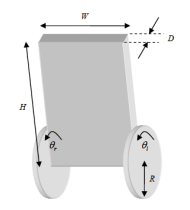
\includegraphics[scale=1.2]{fig1.png}
\end{figure}

\quad A vista lateral e superior deste sistema com as variáveis associadas é mostrada na seguinte
figura:

\begin{figure}[h]
    \centering
    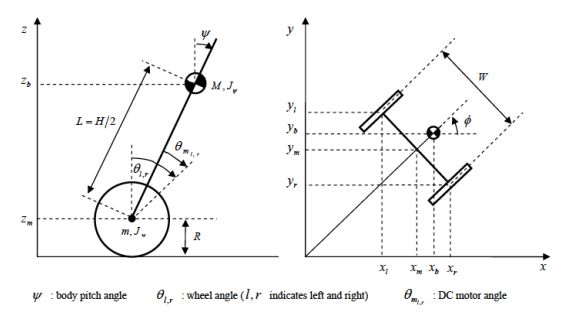
\includegraphics[scale=1.2]{fig2.png}
\end{figure}

\quad Os parâmetros físicos deste sistema são dados por:

\begin{itemize}
    \item $g = 9.8 \text{m/s}^2$: gravidade
    \item $m = 0.03 \text{kg}$: peso da roda
    \item $R = 0.04 \text{m}$: raio da roda
    \item $J_W = \frac{m R^2}{2}$: momento de inércia da roda
    \item $M = 0.6 \text{kg}$: peso do corpo
    \item $W = 0.14 \text{m}$: largura do corpo
    \item $D = 0.04 \text{m}$: profundidade do corpo
    \item $H = 0.144 \text{m}$: altura do corpo
    \item $L = \frac{H}{2}$: distância do centro de massa do corpo ao eixo da roda
    \item $J_{\psi} = \frac{ML^2}{3} \text{kgm}^2$: momento de inércia do corpo em pitch
    \item $J_{\phi} = \frac{M(W^2 + D^2)}{12} \text{kgm}^2$: momento de inércia do corpo em rumo
    \item $J_m$: inércia do motor DC desprezível
    \item $R_m = 6.69 \Omega$: resistência do motor DC
    \item $L_m$: indutância do motor desprezível
    \item $K_t = Ke = 0.4$: constante de torque (Nm/A) e constante de EMF (V s/rad)
    \item $f_m = 0.0022$: atrito entre o corpo e o motor
    \item $n = 1$: redução do motor
\end{itemize}

\quad Considerando os graus de liberdade $\{\theta, \psi, \phi \}$ onde $\theta = (\theta_l + \theta_r)/2 \rightarrow \dot{\theta} = (\dot{\theta_l} + \dot{\theta_r})/2$.

\quad A posição cartesiana do carrinho (composto pelas 2 rodas), no sistema de coordenadas
$\{x, y, x\}$, é dada por:

\begin{equation}
    X_m =
    \begin{bmatrix}
        x_m \\
        y_m \\
        z_m
    \end{bmatrix} =
    \begin{bmatrix}
        x_m \\
        y_m \\
        R
    \end{bmatrix}
\end{equation}

\quad Considerando que as rodas do carrinho não escorregam,
o carrinho é um sistema com restrições não-holonômicas,
sendo que a velocidade do carrinho é dada por:

\begin{equation}
    \dot{X_m} = R
    \begin{bmatrix}
        cos(\phi) \\
        sin(\phi) \\
        0
    \end{bmatrix}
    \dot{\theta}
\end{equation}

\quad A posição cartesiana das rodas (esquerda e direita) no sistema de coordenadas $\{x, y, x\}$,
é dada por:

\begin{equation}
\begin{aligned}
    X_l =
    \begin{bmatrix}
        x_l \\
        y_l \\
        z_l
    \end{bmatrix} =
    X_m + \frac{W}{2}
    \begin{bmatrix}
        - sin(\phi) \\
        cos(\phi) \\
        0
    \end{bmatrix}  \\
    X_r =
    \begin{bmatrix}
        x_r \\
        y_r \\
        z_r
    \end{bmatrix} =
    X_m + \frac{W}{2}
    \begin{bmatrix}
        sin(\phi) \\
        - cos(\phi) \\
        0
    \end{bmatrix}
\end{aligned}
\end{equation}

\quad A velocidade cartesiana das rodas é dada por:

\begin{equation}
    \begin{aligned}
        \dot{X_l} =
        \dot{X_m} + \frac{W}{2}
        \begin{bmatrix}
            - cos(\phi) \\
            - sin(\phi) \\
            0
        \end{bmatrix} \dot{\phi} \\
        \dot{X_r} =
        \dot{X_m} + \frac{W}{2}
        \begin{bmatrix}
            cos(\phi) \\
            sin(\phi) \\
            0
        \end{bmatrix} \dot{\phi}
    \end{aligned}
\end{equation}

\quad A posição cartesiana do corpo no sistema de coordenadas $\{x, y, x\}$,
é dada por:

\begin{equation}
    X_b = 
    \begin{bmatrix}
        x_b \\
        y_b \\
        z_b
    \end{bmatrix} = X_m + L
    \begin{bmatrix}
        cos(\phi) sin(\psi) \\
        sin(\phi) sin(\psi) \\
        cos(\psi)
    \end{bmatrix}
\end{equation}

\quad A velocidade cartesiana do corpo é dada por:

\begin{equation}
    \dot{X_b} = \dot{X_m} + L
    \begin{bmatrix}
        cos(\phi) cos(\psi) \\
        sin(\phi) cos(\psi) \\
        -sin(\psi)
    \end{bmatrix} \dot{\psi} + L
    \begin{bmatrix}
        -sin(\phi) sin(\psi) \\
        cos(\phi) sin(\psi) \\
        0
    \end{bmatrix} \dot{\phi}
\end{equation}

\quad Levando em consideração que a massa do motor DC é desprezível e
utilizando a fórmula de energia cinética translacional de um único corpo,
a energia cinética translacional é dada por:

\begin{equation}
    E_c = \frac{1}{2} m \|\vec{v}\|^2
\end{equation}

\begin{equation}
\begin{gathered}
    T_1 = \frac{1}{2}m \dot{X_l^T} \dot{X_l} +
    \frac{1}{2}m \dot{X_r^T} \dot{X_r} +
    \frac{1}{2}M \dot{X_b^T} \dot{X_b} = \\
    = \frac{1}{2}m
    \begin{bmatrix}
        R cos(\phi) \dot{\theta} - \frac{W}{2}cos(\phi)\dot{\phi}
        & R sin(\phi) \dot{\theta} - \frac{W}{2}sin(\phi)\dot{\phi}
        & 0
    \end{bmatrix}
    \begin{bmatrix}
        R cos(\phi) \dot{\theta} - \frac{W}{2}cos(\phi)\dot{\phi} \\
        R sin(\phi) \dot{\theta} - \frac{W}{2}sin(\phi)\dot{\phi} \\
        0
    \end{bmatrix} + \\
    \frac{1}{2}m
    \begin{bmatrix}
        R cos(\phi) \dot{\theta} + \frac{W}{2}cos(\phi)\dot{\phi}
        & R sin(\phi) \dot{\theta} + \frac{W}{2}sin(\phi)\dot{\phi}
        & 0
    \end{bmatrix}
    \begin{bmatrix}
        R cos(\phi) \dot{\theta} + \frac{W}{2}cos(\phi)\dot{\phi} \\
        R sin(\phi) \dot{\theta} + \frac{W}{2}sin(\phi)\dot{\phi} \\
        0
    \end{bmatrix} + \\
    \scalebox{0.7}{$
    \frac{1}{2}M
    \begin{bmatrix}
        R cos(\phi) \dot{\theta} + L cos(\phi)cos(\psi)\dot{\psi} - L sin(\phi)sin(\psi)\dot{\phi}
        & R sin(\phi) \dot{\theta} + L sin(\phi)cos(\psi)\dot{\psi} + L cos(\phi)sin(\psi)\dot{\phi}
        & -L sin(\psi) \dot{\psi}
    \end{bmatrix}
    \begin{bmatrix}
        R cos(\phi) \dot{\theta} + L cos(\phi)cos(\psi)\dot{\psi} - L sin(\phi)sin(\psi)\dot{\phi}
        \\ R sin(\phi) \dot{\theta} + L sin(\phi)cos(\psi)\dot{\psi} + L cos(\phi)sin(\psi)\dot{\phi}
        \\ -L sin(\psi) \dot{\psi}
    \end{bmatrix} =
    $} \\
    = \frac{1}{2}m \left[R^2cos(\phi)^2\dot{\theta}^2 - WR cos(\phi)^2\dot{\theta}\dot{\phi} + \frac{W^2}{4}cos(\phi)\dot{\phi}^2 + R^2sin(\phi)^2\dot{\theta}^2 - WR sin(\phi)^2\dot{\theta}\dot{\phi} + \frac{W^2}{4}sin(\phi)\dot{\phi}^2\right] + \\
    \frac{1}{2}m \left[R^2cos(\phi)^2\dot{\theta}^2 + WR cos(\phi)^2\dot{\theta}\dot{\phi} + \frac{W^2}{4}cos(\phi)\dot{\phi}^2 + R^2sin(\phi)^2\dot{\theta}^2 + WR sin(\phi)^2\dot{\theta}\dot{\phi} + \frac{W^2}{4}sin(\phi)\dot{\phi}^2\right] + \\
    \frac{1}{2}M \\
    \scalebox{1.1}{$
    = \frac{m \left[R^2\dot{\theta}^2 - WR\dot{\theta}\dot{\phi} + \frac{W^2}{4}\dot{\phi}^2 + R^2\dot{\theta}^2 + WR\dot{\theta}\dot{\phi} + \frac{W^2}{4}\dot{\phi}^2\right] + M \left[ R^2 \dot{\theta}^2 + L^2cos(\psi)^2\dot{\psi}^2 + L^2 sin(\psi)^2 \dot{\phi}^2 + 2RL cos(\psi)\dot{\theta}\dot{\psi} + L^2sin(\psi)^2\dot{\psi}^2 \right]}{2} =
    $}\\
    = \frac{m \left[2R^2\dot{\theta}^2 + \frac{W^2}{2}\dot{\phi}^2\right] + M \left[ R^2 \dot{\theta}^2 + L^2\dot{\psi}^2 + L^2 sin(\psi)^2 \dot{\phi}^2 + 2RL cos(\psi)\dot{\theta}\dot{\psi}\right]}{2}
\end{gathered}
\end{equation}

\section{Derivação e obtenção das equações dinâmicas}

\end{document}